%%%%%%%%%%%%%%%%%%%%%%%%%%%%%%%%%%%%%%%%%%%%%%%%%%%%%%%%%%%%%%%%%%%%%%%%%%%%%%%%
%% Projeto Final de Graduação
%% Aluno: Victor Seixas Souza
%% Orientadora: Christiane Neme Campos
%% Tema: Teoria de Ramsey em Grafos
%%%%%%%%%%%%%%%%%%%%%%%%%%%%%%%%%%%%%%%%%%%%%%%%%%%%%%%%%%%%%%%%%%%%%%%%%%%%%%%%
% !TEX root = ../thesis.tex
%%%%%%%%%%%%%%%%%%%%%%%%%%%%%%%%%%%%%%%%%%%%%%%%%%%%%%%%%%%%%%%%%%%%%%%%%%%%%%%%

\chapter{Números de Ramsey para outros Grafos}
\label{chap:graph}

%%%%%%%%%%%%%%%%%%%%%%%%%%%%%%%%%%%%%%%%%%%%%%%%%%%%%%%%%%%%%%%%%%%%%%%%%%%%%%%%

Uma característica interessante da Teoria de Ramsey é sua capacidade ser generalizada de diversas maneiras. Até agora, sempre consideramos colorações que não tinham o grafo $K_r$ como subgrafo monocromático. Vamos relaxar esta condição e proibir grafos genéricos monocromáticos.

%%%%%%%%%%%%%%%%%%%%%%%%%%%%%%%%%%%%%%%%
\begin{definition}
Sejam $G$ e $H$ grafos simples. Definimos $r(G,H)$ como o menor inteiro positivo $n$, tal que qualquer coloração de arestas em duas cores do grafo $K_n$ possui um $G$ da primeira cor ou um $H$ da segunda cor.
\end{definition}
%%%%%%%%%%%%%%%%%%%%%%%%%%%%%%%%%%%%%%%%

Note que por esta definição, $R(k,s) = r(K_k, K_s)$. Também definimos $r(G) = r(G,G)$. Observemos agora que estes números possuem
Se $G$ é subgrafo de $G'$ então $r(G,H) \leq r(G',H)$. Assim, estes números estão bem definidos pois $r(G,H) \leq r(K_{v(G)}, K_{v(H)}) = R(v(G), v(H)) < \infty$. De maneira analoga, podemos definir os números de Ramsey para várias cores, $r(G_1, \dots, G_k)$, e adaptar a notação $r_k(G) = r(G,\dots,G)$.

Agora vamos estudar algumas classes de grafos interessantes e seus números de Ramsey. Vale observar que mesmo famílias simples de grafos, os números de Ramsey associados podem ser bem difíceis de se determinar. Por este motivo, muitos dos resultados apresentados nesta seção não incluirão as demonstrações. O texto, no entanto, fornece uma base sólida o suficiente para que o leitor interessado, busque as referências e estudem tais demonstrações por si só.

%%%%%%%%%%%%%%%%%%%%%%%%%%%%%%%%%%%%%%%%%%%%%%%%%%%%%%%%%%%%%%%%%%%%%%%%%%%%%%%%

\section{Grafos Bipartidos}

Seja $G = (V,E)$ um grafo simples. Dizemos que $G$ é um \indef{grafo bipartido} se o conjunto $V$ pode ser particionado em duas partes não vazias $X$ e $Y$ de tal forma que toda aresta em $E$ tem uma extremidade em $X$ a outra em $Y$. Tal partição $(X,Y)$ é dita uma \indef{bipartição} do grafo $G$. Um grafo $G$ com bipartição $(X,Y)$ é denotado $G[X,Y]$.

Quando um grafo bipartido $G[X,Y]$ é tal que par de vértices $x \in X$ e $y \in Y$ é adjacente, dizemos que $G[X,Y]$ é um \indef{grafo bipartido completo}. Naturalmente, temos uma família de grafos associada. Denotamos por $K_{n,m}$ o grafo bipartido completo $G[X,Y]$ com $|X| = n$ e $|Y| = m$. Temos portanto que $v(K_{n,m}) = n + m$ e $e(K_{n,m}) = nm$.

%%%%%%%%%%%%%%%%%%%%%%%%%%%%%%%%%%%%%%%%
\begin{figure}[ht!]
\centering
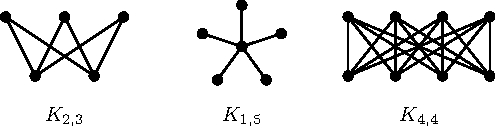
\includegraphics{figures/3_graph_1_part}
\caption{Alguns grafos bipartidos.}
\label{graph:fig:part}
\end{figure}
%%%%%%%%%%%%%%%%%%%%%%%%%%%%%%%%%%%%%%%%

Quando o conjunto de vértices de um grafo pode ser particionado em $k$ partes disjuntas e não vazias de tal forma que nenhuma aresta possui as duas extremidades em uma única parte, dizemos que o grafo é $k$-\emph{partido}. Um grafo bipartido é, portanto, 2-partido. Denotamos por $K_{a_1, \dots, a_k}$ o grafo completo $k$-partido com partes com $a_i$ vértices. Nas próximas seções, mostramos que a família de grafos $k$-partidos completo é bem interessante para construir limitantes inferiores para números de Ramsey.

Um subcaso notável dos grafos bipartidos completos são os \indef{grafos estrela} $K_{1,n}$. O desenho do $K_{1,5}$ na Figura~\ref{graph:fig:part} evidencia a motivação por trás deste nome. Podemos caracterizar os números de Ramsey $r(K_{1,n}, K_{1,m})$ da seguinte forma.

%%%%%%%%%%%%%%%%%%%%%%%%%%%%%%%%%%%%%%%%
\begin{theorem}[Harary~\cite{harary}]
Sejam $n$ e $m$ inteiros positivos, temos que
\[r(K_{1,n}, K_{1,m}) = \begin{cases}
  n + m , & \text{se } n \text{ ou } m  \text{ forem ímpares;} \\
  n + m - 1, & \text{se } m \text{ e } n \text{ forem pares.}
\end{cases}\]
\end{theorem}
%%%%%%%%%%%%%%%%%%%%%%%%%%%%%%%%%%%%%%%%
\begin{proof}
Primeiramente, note que em uma coloração de arestas, um $K_{1,n}$ monocromático na cor $C$ corresponde a um vértice $v$ tal que $d_C(v) \geq n$.

Considere uma $RB$-coloração qualquer de um grafo completo $G$ sem $K_{1,n}$ vermelho ou $K_{1,m}$ azul. Temos então que $d_R(v) \leq n-1$ e $d_B(v) \leq m-1$ para todo vértice $v \in V(G)$. Isto é impossível se $G = K_{n+m}$, logo $r(K_{1,n}, K_{1,m}) \leq n+m$.
Se $m$ e $n$ são pares, considere $G = K_{n+m-1}$. Temos portanto que $d_R(v) = n-1$ e $d_B(v) = m-1$ para todo vértice $v \in V(G)$. Logo, o grafo $G_R$ possui todos os vértices de grau ímpar. Mas $v(G_R) = n + m -1$ também é ímpar. Pelo \emph{handshaking lemma}, não existe grafo com um número ímpar de vértices de grau ímpar. Portanto, $r(K_{1,n}, K_{1,m}) \leq n + m - 1$.

No caso de algum entre $n$ e $m$ ser ímpar, considere sem perda de generalidade que $n$ é ímpar, com $n = 2k + 1$. Considere $G  = K_{n+m-1}$ com $V(G) = \{ v_0, \dots, v_{n+m-1} \}$. Defina uma $RB$-coloração $c$ da seguinte maneira.
\[c(v_i v_j) = \begin{cases}
  \text{vermelho}, & \text{se }  i - j \in \{ -k, \dots, k\} \Mod{n+m-1}; \\
  \text{azul}, & \text{caso contrário}.
\end{cases}\]
Note que nesta coloração, $d_R(v) = 2k = n - 1$ e $d_B(v) = m - 1$ para todo vértice $v \in V(G)$. Portanto, $c$ não possui $K_{1,n}$ vermelho nem $K_{1,m}$ azul, o que implica em $r(K_{1,n}, K_{1,m}) = n + m$.

Suponha agora que ambos $n$ e $m$ são pares. Considere um grafo bipartido $G = G[X,Y]$, com $X = \{ x_i : i \in \Z{l} \}$ e $Y = \{ y_i : i \in \Z{l} \}$, tal que os vértices $x_i$ e $y_j$ são adjacentes se e somente se $i - j \in \{ 1, \dots, k\} \Mod{l}$. Note que $G$ é $k$-regular, e seu complemento é $(2l - k - 1)$-regular.
Escolhendo $l = \frac{n + m -2}{2}$ e $k = n-1$, temos que $G$ é um grafo com $n + m - 2$ vértices que é $(n-1)$-regular com complementar $\comp{G}$ $(m-2)$-regular. Isto corresponde a uma coloração de $K_{n + m - 2}$ sem $K_{1,n}$ vermelho nem $K_{1,m}$ azul. Portanto, temos $r(K_{1,n}, K_{1,m}) = n + m - 1$.
\end{proof}
%%%%%%%%%%%%%%%%%%%%%%%%%%%%%%%%%%%%%%%%

Este resultado pode ser generalizado com idéias parecidas para o número de Ramsey com diversas cores.

%%%%%%%%%%%%%%%%%%%%%%%%%%%%%%%%%%%%%%%%
\begin{theorem}[Burr, Roberts~\cite{burr1973ramsey}]
Sejam $m_1, \dots, m_k$ inteiros positivos, $t$ dos quais são pares. Temos que
\[r(K_{1,m_1}, \dotsc,  K_{1,m_k}) = \sum_{i=1}^{k} m_i  - k + \varepsilon,\]
onde $\varepsilon = 1$ se $t$ é par e $\varepsilon = 2$ caso contrário.
\end{theorem}
%%%%%%%%%%%%%%%%%%%%%%%%%%%%%%%%%%%%%%%%

%%%%%%%%%%%%%%%%%%%%%%%%%%%%%%%%%%%%%%%%%%%%%%%%%%%%%%%%%%%%%%%%%%%%%%%%%%%%%%%%

\section{Caminhos e Ciclos}

Um \indef{caminho} é um grafo simples que pode ter seus vértices listados por uma sequência de modo que dois vértices são adjacentes, se e somente se, correspondem a elementos consecutivos na sequência. Similarmente, um \indef{ciclo} é um grafo simples com $n \geq 3$ que pode ter seus vértices listados por uma seqência cíclica de modo que dois vértices são adjacemtes, se e somente se, correspondem a elementos consecutivos na sequência.

Estas definições evocam naturalmente uma família de grafos associada. Definimos os \indef{grafos caminhos} $P_n$ são os grafos com $n$ vértices e $n-1$ arestas que são isomorficos ao grafo $(\{v_1,\dots,v_n\}, \{v_iv_{i+1}\})$. Adicionando a aresta $v_nv_1$ ao grafo anterior, obtemos os \indef{grafos ciclo} $C_n$, com $n$ vértices e $n$ arestas. Ambas as famílias estão exemplificadas na Figura~\ref{graph:fig:cyclepath}.

%%%%%%%%%%%%%%%%%%%%%%%%%%%%%%%%%%%%%%%%
\begin{figure}[ht!]
\centering
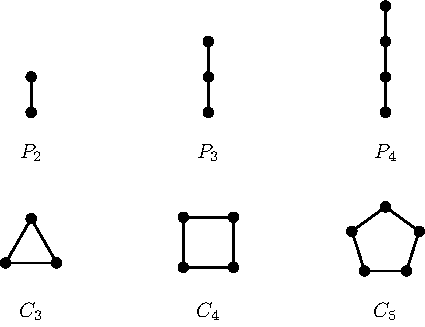
\includegraphics{figures/3_graph_2_cyclepath}
\caption{Alguns ciclos e caminhos pequenos.}
\label{graph:fig:cyclepath}
\end{figure}
%%%%%%%%%%%%%%%%%%%%%%%%%%%%%%%%%%%%%%%%

Se $n > 1$, o grafo $P_n$ possui $2$ vértices de grau um, chamados de \indef{extremidades}, os demais $n-2$ vértices são ditos \indef{internos}, e possuem grau dois. Já o grafo $C_n$ é 2-regular, isto é, possui todos os vértices com grau igual a dois.

O número de Ramsey

%%%%%%%%%%%%%%%%%%%%%%%%%%%%%%%%%%%%%%%%
\begin{theorem}[Gerencsér, Gyárfás~\cite{gerencser1967ramsey}]
Sejam $n \geq m \geq 2$ inteiros, então
\[r(P_n, P_m) = n + \left \lfloor \frac{m}{2} \right \rfloor - 1.\]
\end{theorem}
%%%%%%%%%%%%%%%%%%%%%%%%%%%%%%%%%%%%%%%%

Seja $G$ um grafo simples. Dizemos que dois vértices $x$ e $y$ estão conectados se existe um caminho em $G$ com uma extremidade em $x$ e outra em $y$. Note que esta relação é uma relação de equivalência no conjunto $V(G)$. Chamamos as classes de equivalência desta relação de \indef{componentes}. Dizemos que $G$ é \indef{conexo} se entre quaisquer dois vértices de $G$ estão conectados, ou seja, $G$ possui apenas uma componente.

%%%%%%%%%%%%%%%%%%%%%%%%%%%%%%%%%%%%%%%%
\begin{proposition}
\label{graph:thm:rpt} $r(P_k, K_3) = 2k - 1$.
\end{proposition}
%%%%%%%%%%%%%%%%%%%%%%%%%%%%%%%%%%%%%%%%
\begin{proof}
Note que o
\end{proof}
%%%%%%%%%%%%%%%%%%%%%%%%%%%%%%%%%%%%%%%%

\section{Árvores}









%%%%%%%%%%%%%%%%%%%%%%%%%%%%%%%%%%%%%%%%%%%%%%%%%%%%%%%%%%%%%%%%%%%%%%%%%%%%%%%%


%%%%%%%%%%%%%%%%%%%%%%%%%%%%%%%%%%%%%%%%%%%%%%%%%%%%%%%%%%%%%%%%%%%%%%%%%%%%%%%%
